\documentclass[journal]{IEEEtran}
\usepackage[a5paper, margin=10mm, onecolumn]{geometry}
%\usepackage{lmodern} % Ensure lmodern is loaded for pdflatex
\usepackage{tfrupee} % Include tfrupee package

\setlength{\headheight}{1cm} % Set the height of the header box
\setlength{\headsep}{0mm}     % Set the distance between the header box and the top of the text

\usepackage{gvv-book}
\usepackage{gvv}
\usepackage{cite}
\usepackage{amsmath,amssymb,amsfonts,amsthm}
\usepackage{algorithmic}
\usepackage{graphicx}
\usepackage{textcomp}
\usepackage{xcolor}
\usepackage{txfonts}
\usepackage{listings}
\usepackage{enumitem}
\usepackage{mathtools}
\usepackage{gensymb}
\usepackage{comment}
\usepackage[breaklinks=true]{hyperref}
\usepackage{tkz-euclide} 
\usepackage{listings}
% \usepackage{gvv}                                        
\def\inputGnumericTable{}                                 
\usepackage[latin1]{inputenc}                                
\usepackage{color}                                            
\usepackage{array}                                            
\usepackage{longtable}                                       
\usepackage{calc}                                             
\usepackage{multirow}                                         
\usepackage{hhline}                                           
\usepackage{ifthen}                                           
\usepackage{lscape}
\begin{document}

\bibliographystyle{IEEEtran}
\vspace{3cm}

\title{10.3.1.1}
\author{EE24BTECH11001 - Aditya Tripathy}
 \maketitle
% \newpage
% \bigskip
{\let\newpage\relax\maketitle}

\renewcommand{\thefigure}{\theenumi}
\renewcommand{\thetable}{\theenumi}
\setlength{\intextsep}{10pt} % Space between text and floats


\numberwithin{equation}{enumi}
\numberwithin{figure}{enumi}
\renewcommand{\thetable}{\theenumi}


\textbf{Question}:\\
Aftab tells his daughter, "Seven years ago, I was seven times as old as you were then.
Also, three years from now, I shall be three times as old as you will be.". Represent
this situation algebraically and graphically.
\\
\textbf{Solution: }\\
Let Aftab's present age be denoted by $x$ and his daughter's present age be denoted as $y$.
Now the problem can be represented algebraically as follows :
\begin{align}
    \brak{x-7} = 7\brak{y-7}\\
    \brak{x+3} = 3\brak{y+3}
\end{align}
Simplifying and using matrix notation,
\begin{align}
    x -7y = -42\\
    x - 3y = 6\\
    \myvec{
        1 & -7\\
        1 & -3
    } \myvec{x \\ y}= \myvec{ -42 \\ 6}
\end{align}

Any non-sigular matrix can be represented as a product of a lower triangular matrix $L$ and an
upper triangular matrix $U$

\begin{align}
    A\vec{x} = LU\vec{x} = \vec{b}
\end{align}
The upper triangular matrix U is found by row reducing A,
\begin{align}
    \myvec{1 & -7 \\ 1 & -3 } \xrightarrow{R_2 -> R_2 - R_1} \myvec{1 & -7 \\ 0 & 4}  
\end{align}
Let 
\begin{align}
    L = \myvec{1 & 0\\ l_{21} & 1}
\end{align}
$l_{21}$ is the multiplier used to zero $a_{21}$, so $l_{21} = 1$.\\
\newline
Now,
\begin{align}
    A = \myvec{1 & -7 \\ 1 & -3} = \myvec{1 & 0 \\ 1 & 1}\myvec{1 & -7 \\ 0 & 4}
\end{align}
Now we can get the solution to our problem by the two step process,
\begin{align}
    L\vec{y} = \vec{b}\\
    U\vec{x} = \vec{y}
\end{align}
Using forward substitution to solve the first equation,
\begin{align}
    \myvec{1 & 0 \\ 1 & 1}\myvec{y_1 \\ y_2} &= \myvec{-42 \\ 6}\\
    \xrightarrow{} \myvec{y_1 \\ y_2} &= \myvec{-42 \\ 48} 
\end{align}
Now using back-substitution for the second equation,
\begin{align}
    \myvec{1 & -7 \\ 0 & 4}\myvec{x_1 \\ x_2} &= \myvec{-42 \\ 48}\\
    \myvec{x_1 \\ x_2} &= \myvec{42 \\ 12}
\end{align}
Therefore Aftab's age is 42 years and 12 years is the age of his daughter.
\begin{figure}[h!]
   \centering
   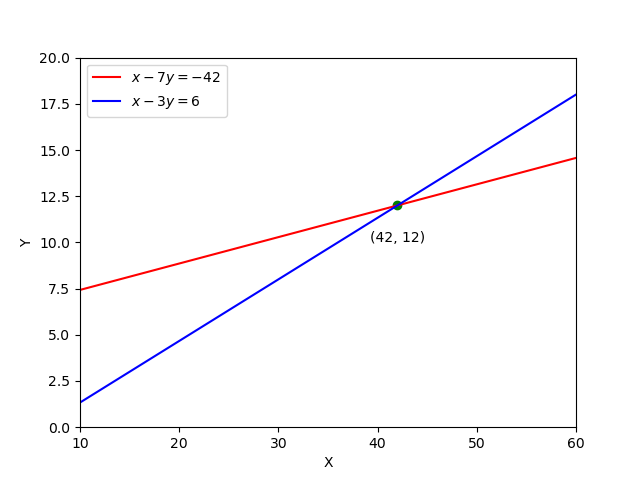
\includegraphics[width=0.7\columnwidth]{figs/fig.png}
    \caption{Solution to set of linear equations}
\end{figure}
\end{document}
